% Figure F1 — Chaîne de transmission en bande de base (TS227, chapitre 2).
% D'après le support [poly, p. 19], redessinée.
% Rendu SVG :
%   latex -output-directory=<dossier temporaire> 02-chaine-bande-de-base.tex
%   dvisvgm --no-fonts --exact-bbox -o 02-chaine-bande-de-base.svg <dossier temporaire>/02-chaine-bande-de-base.dvi
\documentclass[tikz,border=4pt]{standalone}
\usepackage[T1]{fontenc}
\usepackage[utf8]{inputenc}
\usepackage{sansmath}
\renewcommand{\familydefault}{\sfdefault}
\usetikzlibrary{positioning,arrows.meta,calc,fit}
\begin{document}
\sansmath
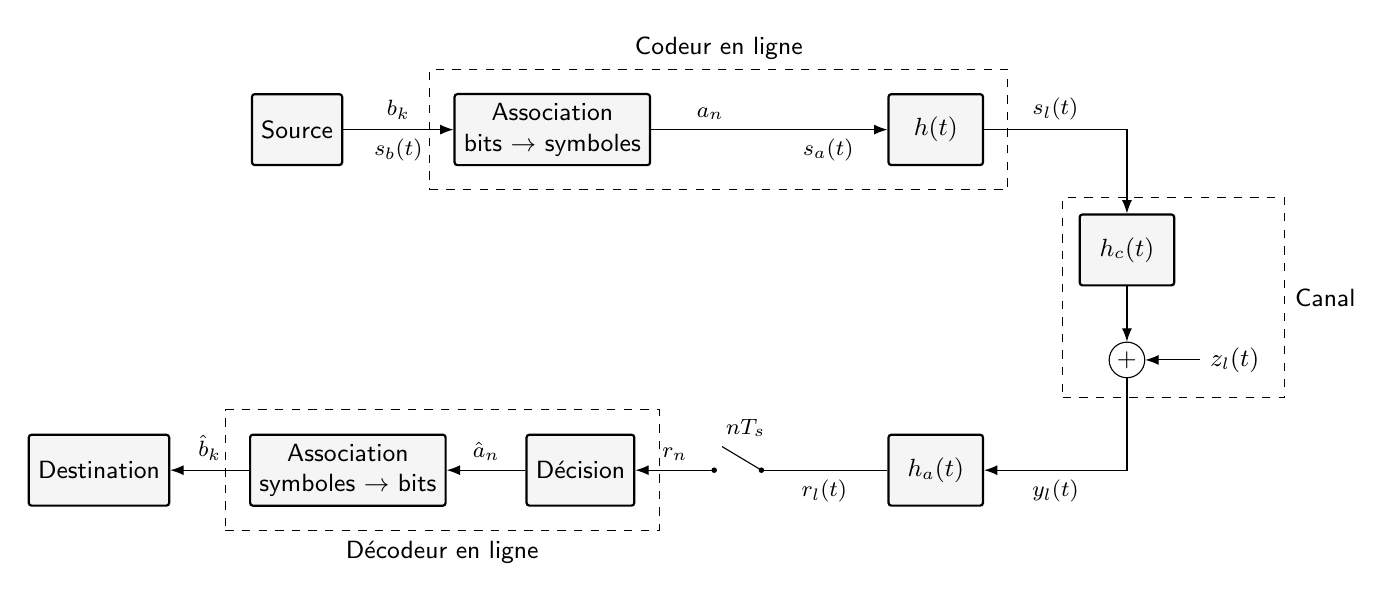
\begin{tikzpicture}[
    >=Latex, font=\small,
    bloc/.style={draw, thick, rounded corners=1pt, minimum height=9mm, align=center, fill=black!4},
    filtre/.style={bloc, minimum width=12mm},
    groupe/.style={draw, dashed, inner sep=3mm},
    sig/.style={font=\footnotesize},
  ]
  % --- Émission (ligne du haut) ---
  \node[bloc] (src) {Source};
  \node[bloc, right=14mm of src] (assoc) {Association\\bits $\to$ symboles};
  \node[filtre, right=30mm of assoc] (h) {$h(t)$};
  % --- Canal ---
  \node[filtre, below right=6mm and 12mm of h] (hc) {$h_c(t)$};
  \node[draw, circle, inner sep=1.2pt, below=7mm of hc] (plus) {$+$};
  \node[right=7mm of plus] (zl) {$z_l(t)$};
  % --- Réception (ligne du bas) ---
  \node[filtre] (ha) at (h |- plus) [yshift=-14mm] {$h_a(t)$};
  \coordinate (ech) at ($(ha.west)+(-22mm,0)$);
  \node[bloc, left=10mm of ech] (dec) {Décision};
  \node[bloc, left=10mm of dec] (associnv) {Association\\symboles $\to$ bits};
  \node[bloc, left=10mm of associnv] (dst) {Destination};

  % Liaisons émission
  \draw[->] (src) -- node[above, sig] {$b_k$} node[below, sig] {$s_b(t)$} (assoc);
  \draw[->] (assoc) -- node[above, sig, pos=0.25] {$a_n$} node[below, sig, pos=0.75] {$s_a(t)$} (h);
  \draw[->] (h.east) -- node[above, sig] {$s_l(t)$} (hc |- h.east) -- (hc.north);
  % Canal
  \draw[->] (hc) -- (plus);
  \draw[->] (zl) -- (plus);
  \draw[->] (plus.south) |- node[below, sig, pos=0.75] {$y_l(t)$} (ha.east);
  % Réception : filtre, échantillonneur (interrupteur), décision
  \draw (ha.west) -- node[below, sig] {$r_l(t)$} ($(ech)+(6mm,0)$);
  \fill ($(ech)+(6mm,0)$) circle (1pt);
  \draw ($(ech)+(6mm,0)$) -- ++(-5mm,3mm);
  \node[sig, above] at ($(ech)+(4mm,3mm)$) {$nT_s$};
  \fill ($(ech)$) circle (1pt);
  \draw[->] (ech) -- node[above, sig] {$r_n$} (dec);
  \draw[->] (dec) -- node[above, sig] {$\hat{a}_n$} (associnv);
  \draw[->] (associnv) -- node[above, sig] {$\hat{b}_k$} (dst);

  % Groupes
  \node[groupe, fit=(assoc)(h), label={above:Codeur en ligne}] {};
  \node[groupe, fit=(hc)(plus)(zl), inner sep=2mm, label={right:Canal}] {};
  \node[groupe, fit=(dec)(associnv), label={below:Décodeur en ligne}] {};
\end{tikzpicture}
\end{document}
